\documentclass{article}
\author{Max Springenberg}
\title{GTI B01}
\usepackage{amsmath}
\usepackage{amssymb}
\usepackage{stmaryrd}
\usepackage{graphicx}
\setcounter{section}{1}

\begin{document}
\maketitle
\newpage

\subsection{Regulaere Ausdruecke}
\subsubsection{Kurzaufgabe}
mit:\\
$
a^* = $"kein a oder mehrere aufeinanderfolgende"$\\
a^+ = $"ein a oder mehrere aufeinanderfolgende"$\\
$
\\
folgt:\\
$
(ab^+)^+ \equiv (abb^*)(abb^*)\\
$
\subsubsection{Hauptaufgabe}
(a)\\
Umbennungen machen bei komplexeren Ausdruecken Sinn, hier ist
es nur Zierde.\\
Eine Umbennenung u sei wie folgt definiert:\\
$
u(+) = +\\
u(*) = *\\
u(V^{operant}) = u(V)^{u(operant)}\\
u(V) = \neg V\\
$mit $\neg 1 = 0,\ \neg 0 = 1\\
$
\\
So gilt fuer die Gesuchte Menge $L'$:\\
$
%\alpha_1 = (01^*)(((00)^+0^*) + (0^+1^*0^+))(0^*1^*)^*\\
\alpha_1 = (01^*)^3\\
\alpha_2 = (10^*)^3 \equiv u(\alpha_1)\\
L' = L(\alpha_1 + \alpha_2)\\
$
\\
(b)\\
Alphabet:\\
$
\Sigma = \{\Sigma_1, \Sigma_2, \Sigma_3\}\\
\Sigma_1 = \{a,...,z\}\\
\Sigma_2 = \{A,...,Z\}\\
\Sigma_3 = \{0,...,9\}\\
$Es gelte des weiteren:$\\
a \in \Sigma_1, b \in \Sigma_2, c \in \Sigma_3\\
\\
(i)\\
\alpha = a^+c(a^*b^*c^*)^* + b^+c(a^*b^*c^*)^*\\
M_1 = L(\alpha)\\
\\
(ii)\\
\beta = (c^+(a^*b^*c^*)^*) 
        + (a^*b^*)^* 
        + (ba + (a^*b^*c^*)^*)
        + (ab + (a^*b^*c^*)^*)\\
M_2 = L(\beta)\\
$

\newpage
\subsection{Deterministische endliche Automaten}
\subsubsection{Kurzaufgabe}
Startzustand ist der Einzige Akzeptierendenzustand $q_0$.\\
Der Automat summiert solange Zahlen aus dem Eingabeaphabet, bis sie
durch 3 ganz teilbar sind, bevor er wieder in den akzeptierenden 
Zustand wechselt.\\
\\
ZustandsMenge:\\$
Q = \{q_0, q_1, q_2\}\\
\\
$EingabeAlphabet:\\$
\Sigma = \{0,...,9\}\\
\\
$Transitionsfunktion:\\$
\delta(p_0, w) =
\begin{cases}
    q_0&\text{wenn }w \equiv_3 0\\
    q_1&\text{wenn }w \in \{1,4,7\}\\
    q_2&\text{sonst}\\
\end{cases}\\
\delta(p_1, w) =
\begin{cases}
    q_0&\text{wenn }w \in \{2,5,8\}\\
    q_1&\text{wenn }w \equiv_3 0\\
    q_2&\text{sonst}\\
\end{cases}\\
\delta(p_2, w) =
\begin{cases}
    q_0&\text{wenn }w \in \{1,4,7\}\\
    q_1&\text{wenn }w\in \{2,5,8\}\\
    q_2&\text{sonst}\\
\end{cases}\\
\\
$Akzeptierte Zustaende:\\$
F = \{q_0\}\\
$
\subsubsection{Hauptaufgabe}
(a)\\
Der Automat kann nur Werte aus dem Eingabealphabet der Zweielementigen
Menge auswerten. Startzustand ist $q_0$, sobald $q_0$ eine 0 uebergeben
wird verweilt der Automat fuer alle folgenden Eingaben im einzigen 
akzeptierenden Zustand $q_2$. wird $q_0$ eine 1 uebergeben so wechselt 
der Automat in den Zustand $q_1$, welcher dann wieder unabhangig der 
Eingabe in $q_0$ wechselt.\\
Fuer die Sprache bedeutet dies, dass mindestens eine 0 in einem Wort enthalten
sein muss.\\
\\
(b)\\
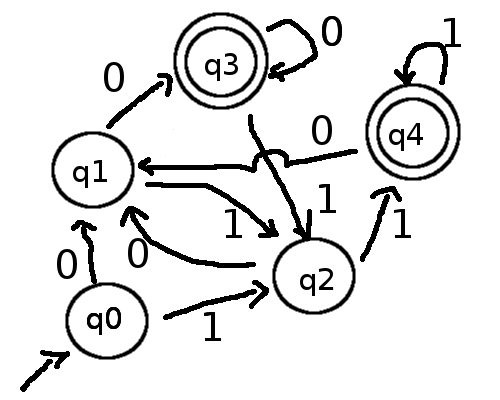
\includegraphics[height=5cm]{./UB1/2b.png}\\
\\
(c)\\
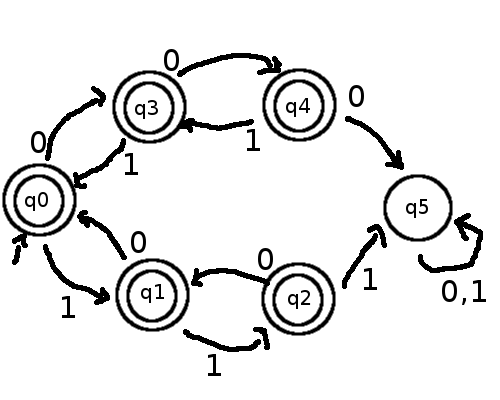
\includegraphics[height=5cm]{./UB1/2c.png}\\

\newpage
\subsection{Endliche Automaten}
\subsubsection{Kurzaufgabe}
\subsubsection{Hauptaufgabe}
(a)\\
\\
(b)\\
\end{document}
